%% ****** Start of file template.aps ****** %
%%
%%
%%   This file is part of the APS files in the REVTeX 4 distribution.
%%   Version 4.0 of REVTeX, August 2001
%%
%%
%%   Copyright (c) 2001 The American Physical Society.
%%
%%   See the REVTeX 4 README file for restrictions and more information.
%%
%
% This is a template for producing manuscripts for use with REVTEX 4.0
% Copy this file to another name and then work on that file.
% That way, you always have this original template file to use.
%
% Group addresses by affiliation; use superscriptaddress for long
% author lists, or if there are many overlapping affiliations.
% For Phys. Rev. appearance, change preprint to twocolumn.
% Choose pra, prb, prc, reverprd, pre, prl, prstab, or rmp for journal
%  Add 'draft' option to mark overfull boxes with black boxes
%  Add 'showpacs' option to make PACS codes appear
\documentclass[aps,prl,twocolumn,superscriptaddress,groupedaddress]{revtex4}  % for review and submission
%\documentclass[aps,preprint,showpacs,superscriptaddress,groupedaddress]{revtex4}  % for double-spaced preprint
\usepackage{graphicx}  % needed for figures
\usepackage{dcolumn}   % needed for some tables
\usepackage{bm}        % for math
\usepackage{amssymb}   % for math

% avoids incorrect hyphenation, added Nov/08 by SSR
\hyphenation{ALPGEN}
\hyphenation{EVTGEN}
\hyphenation{PYTHIA}

\begin{document}

% The following information is for internal review, please remove them for submission
\widetext
\leftline{Version 1.3 as of \today}
%\leftline{Primary authors: Joe E. Physics}
%\leftline{To be submitted to (PRL, PRD-RC, PRD, PLB; choose one.)}
%\leftline{Comment to {\tt d0-run2eb-nnn@fnal.gov} by xxx, yyy}
%\centerline{\em D\O\ INTERNAL DOCUMENT -- NOT FOR PUBLIC DISTRIBUTION}

% the following line is for submission, including submission to the arXiv!!
%\hspace{5.2in} \mbox{Fermilab-Pub-04/xxx-E}

\title{Investigation of MHD Mode Structure in Shaped HBT-EP Plasmas}

%\input author_list.tex       % D0 authors (remove the first 3 lines
                             % of this file prior to submission, they
                             % contain a time stamp for the authorlist)
                             % (includes institutions and visitors)
\date{\today}


\begin{abstract}
Magneto-hydrodynamic (MHD) instabilities can limit the performance of tokamak plasmas, and control of MHD instabilities depends on accurate measurement and understanding of mode structure.  Until the present time, the HBT-EP plasma has been circular in cross section, while the main thrust of research towards a fusion reactor is focused on plasmas that are shaped.  Calculations of ideal MHD instability predict modifications to the mode structure when HBT-EP discharges are shaped\cite{Maurer}.  This dissertation investigates the effect by using a newly installed poloidal field coil which shapes the high field side of the plasma, and can impose a poloidal field null.  Initial measurements of shaped plasmas show a modification to the mode structure consistent with predictions.
\end{abstract}

\maketitle
\section{Introduction}
The kink mode is a performance limiting, disruptive MHD instability\cite{Strait}.  These modes can be driven by either pressure or current gradients, and they have a variety of mode structures depending upon flux surface shape and current and pressure profiles.  The external kink mode is seen in all tokamaks at sufficiently high plasma pressure.  Under certain conditions, the kink mode presents as the resistive wall mode (RWM) as nearby conducting structures' eddy currents limit the growth rate to their resistive time scale.  If the kink has a high rotational frequency, the eddy decay will be negligible and the mode behavior will approach that of an ideal, wall-stabilized, kink.  Kink instabilities are characterized by a dominant poloidal and toroidal wave numbers m and n.  HBT-EP generally presents low-n kinks, the strongest of which are those with ratio m/n just below the helicity of the edge magnetic field\par
	Shaping a plasma has been shown to allow access to higher $\beta$ operating regimes as well as easier access to high confinement regimes (H-mode)\citep{Lazarus, Keilhacker_HMode}. Shaping a plasma is also necessary to direct the large heat flux of a fusion plasma into a divertor designed to safely accept it.  As such, most modern high-performance tokamaks operate diverted, as will ITER.  However, as the equilibrium surface of the plasma changes, so will the shape, and possibly the behavior of the unstable kink mode.  Simulations of ITER-like plasmas have predicted a range of effects on the kink mode in an H-mode diverted plasma, from a strong suppressive effect on current driven kinks coupled with the growth of a distinct new kink/tearing mode\cite{Huysmans} to a change in the mode shape and stability as edge q* varies\cite{Maurer}.\par
%This effect can be seen in a current-driven model as well.  Figure \ref{DCON_dW} a) shows how the two least stable mode energies vary with q*, which is varied by changing plasma current, in the presence and absence of shaping.  q* is calculated on HBT-EP using MR and Ip measurements and a circular, cylindrical approximation, which is invalid in the case of a diverted plasma, as seen in b). q* is calculated in this case by using the (1+$\kappa$) correction for an elongated plasma and is seen to be quite different than our equilibrium measurements and circular approximation would suggest.  Mode mixing occurs in limited plasmas at integer q* as the least stable mode changes shape.  We would expect to see a clean mode with a narrow FFT spectrum when the two modes are widely separated, and a mixed mode with a broad spectrum when they come together.  This would be difficult in circular limited plasmas, as both modes are expected to be stable at the crossover.  By contrast, in diverted plasmas, we see that at low current (high q*) there is an unstable mode and a marginally stable mode, which meets the Boozer criterion for n=1 multimode\cite{Boozer}.  Shaping is seen to change the q* values at which the modes exchange stability, and the n=1 multimode region is seen at a q* of ~2.6, rather than an integer value.  Equilibrium values in 2 a) and b) are chosen such that the the plasma is always diverted.  TokaMac and DCON can not integrate to a separatrix, and output, including q* and mode energetics, is seen to be a weak function of how close to the edge the calculation takes place. Fig 2c), however, shows that even in shaped but limited plasmas, i.e. fully simulated to the last closed flux surface (LCFS), the energetics of an equilibrium are seen to vary with shaping.\par
		
\begin{figure}[b]
	\centering
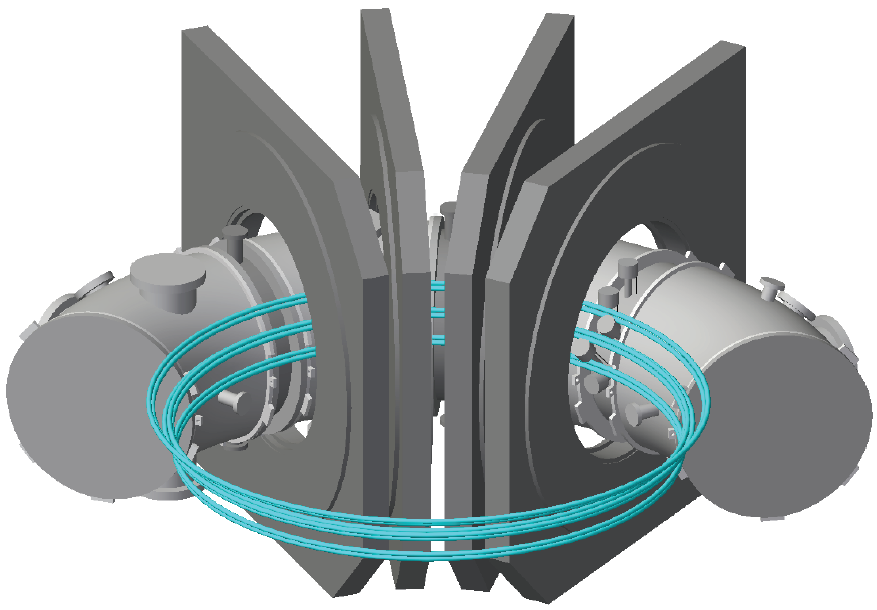
\includegraphics[scale=.35]{../Plots/HBT_section_cropped.png}\caption{Section of HBT-EP, shaping coil shown in blue}
	\label{Coil_HBT_Section}
	\end{figure}
		
\begin{figure*}[htb]
	\centering
	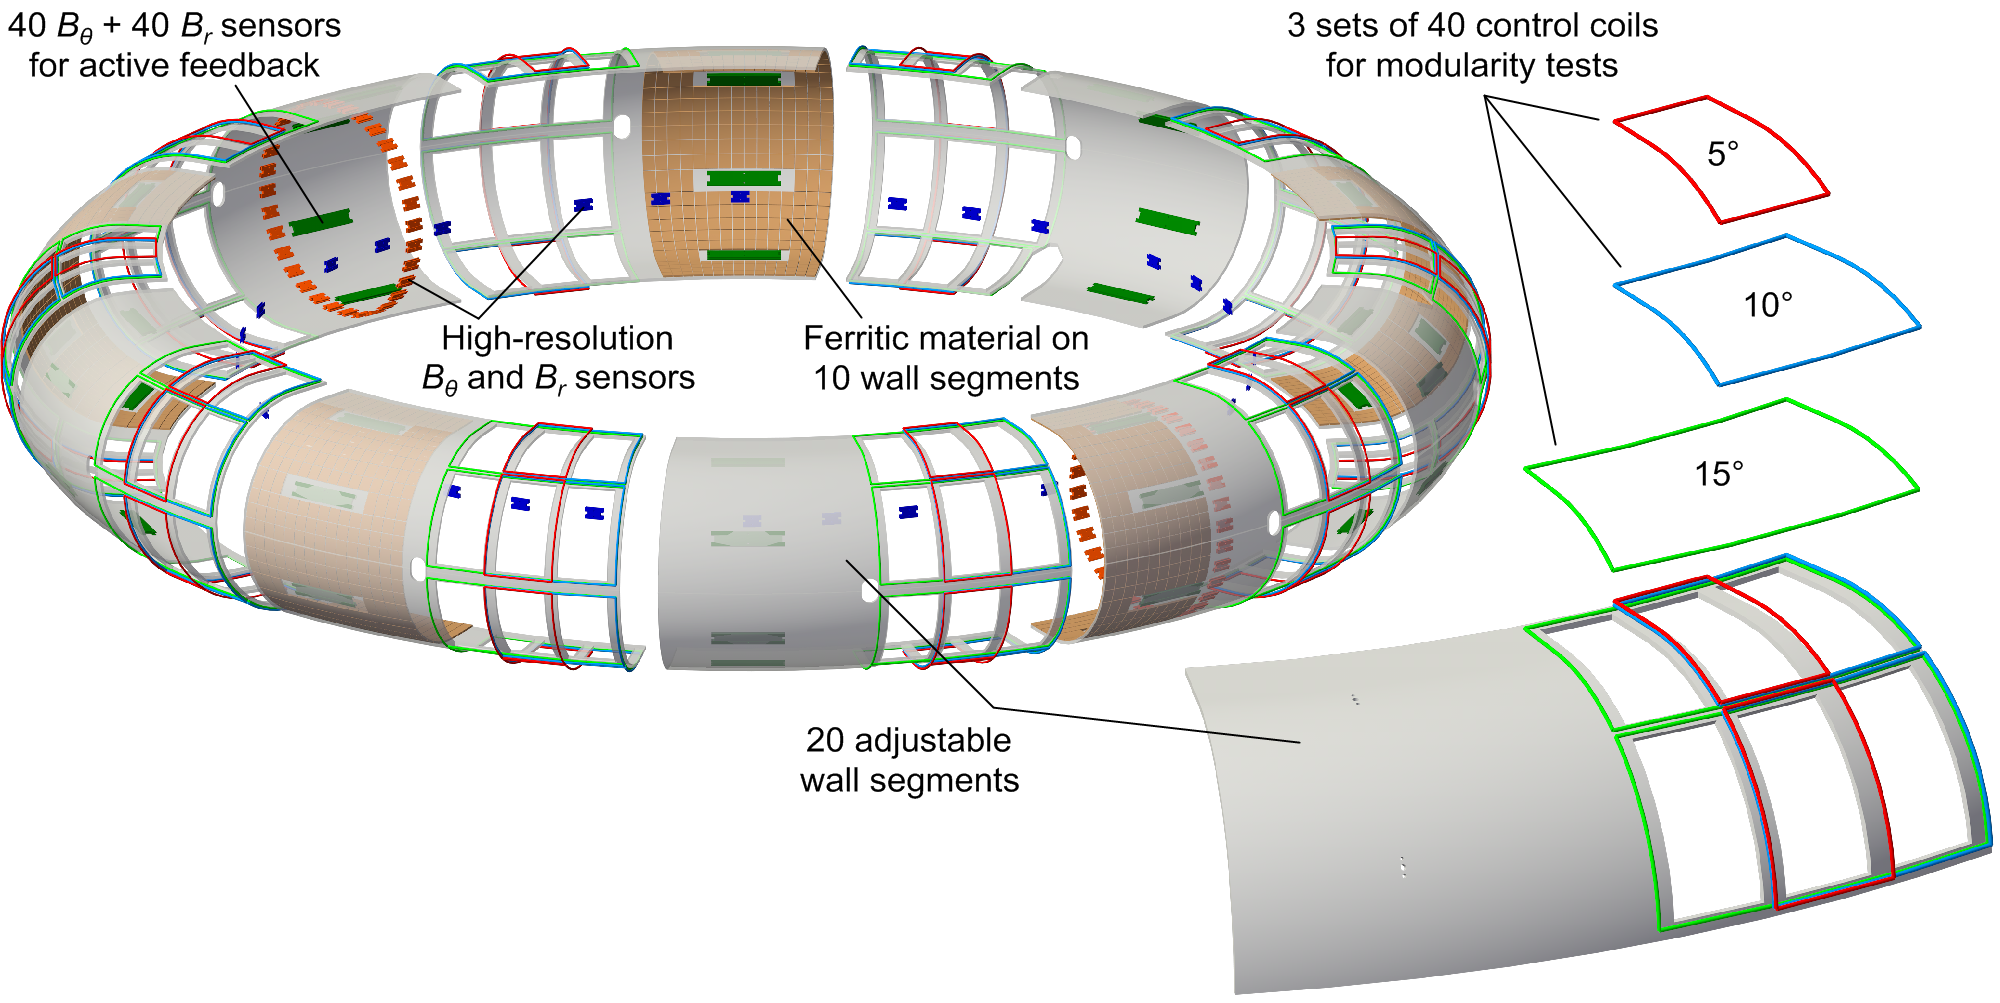
\includegraphics[scale=.25]{../Plots/Plasma_with_sensors_FWall_concept_WithCCview.png}
	\caption{Rendering of the HBT-EP magnetic diagnostics.  Chamber and shell mounted sensor arrays are used to observe and diagnose natural and driven modes MHD.  Passively stabilizing shells and active control coils of various sizes are used to feed back on the modes.  Ferritic sections are retracted for shaping experiments}
	\label{schematic}
	\end{figure*}
	
\begin{figure*}[t]
	\centering
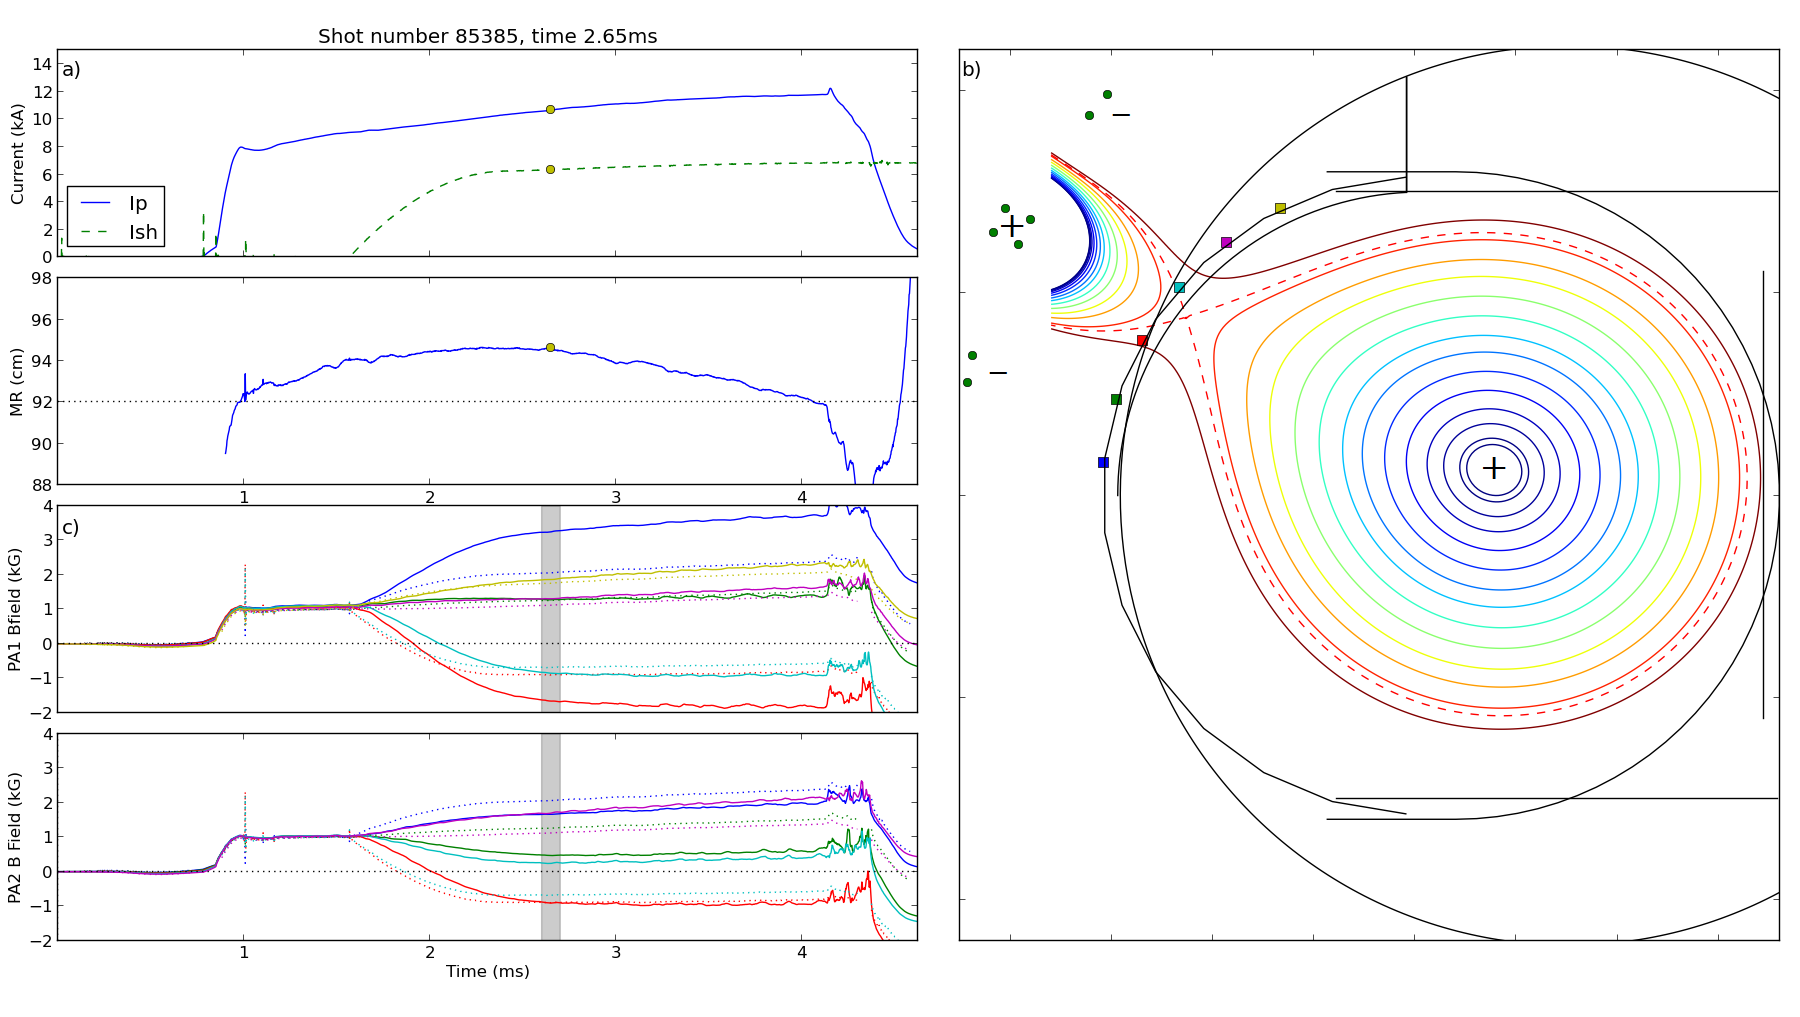
\includegraphics[scale=.4]{../Plots/shot_85388_currents_fields_fluxes_better_aspect_ratio_polarity.png}\caption{HBT-EP shot 85385, including: \\a) Equlibrium measurements of $I_p$, $I_{Shape}$ and MR.\\  b) TokaMac equilibrium reconstruction of flux surfaces, including plasma and coil polarities\\c) Sensor measurements of Bp near the x-point, compared to expected values (dotted lines).\\  Sensor locations are shown in b), traces are color coded to their sensor.\\}
	\label{fluxes and fields}
\end{figure*}

%\begin{widetext}
%This is a test of twocolumn false
%\end{widetext}

\section{The HBT-EP Tokamak}
	HBT-EP is well suited to study the MHD consequences of shaping, as its research mission encompasses the RWM and multimode MHD, and so is well instrumented to detect, analyze and excite MHD activity.  It also has a highly flexible configuration allowing study of MHD in multiple regimes(see Figure \ref{schematic}). It is with this in mind that a zero-net-turns coil has been constructed and installed on HBT-EP for the purposes of this thesis.  It locally shapes the plasma roughly 30${^\circ}$ above the inboard midplane, and is capable of diverting the plasma at this location.
\subsection{The Shaping Coil}
    The Shaping Coil is HBT-EP's newest vacuum field coil.  Installed over the summer and autumn of 2012, it shapes the plasma using a quadrupole poloidal field created by three counterwound coil bundles.  Positioned outside the vacuum vessel at the inboard side of the torus just above the midplane, or ~150$^{\circ}$ of poloidal angle, it imposes an X-point on a line between the central bundle and the plasma center.  The X-point can be pushed into the chamber, thus diverting the plasma, or conditions can be chosen such that the X-point remains behind the material limters, leaving the plasma shaped but limited.\par
    The coil is a single continuous conductor wound in both the co- and contra-IP direction forming a 'zero-net-turns' divertor similar to that used in ASDEX-Upgrade\cite{Keilhacker}.  The coil's field decays rapidly in r and $\theta$, ensuring that the shaping of the plasma is highly localized in radius and poloidal angle.  To allow good coupling, the coil required construction as close as possible to the plasma, inside the TF coils and just outside the inboard edge of the vacuum vessel (see Figure \ref{Coil_HBT_Section}).\par
This coil is powered by a two-stage capacitive power bank, similar in operation to those used to power HBT-EP's other electromagnets\cite{Gates}. A low capacitance, high voltage startup supply discharges quickly to initialize the pulse, and a high capacitance, low voltage crowbar supply sustains the discharge current for the life of the plasma.  The shaping coil's field is nearly constant in time after after a fast ramp - though the capability exists to have it start slowly and ramp with $I_p$ - and is a significant fraction of poloidal field due to $I_p$.  The crowbar bank is passively switched into the system through a diode, greatly simplifying the construction and control of the bank, and ensuring a smooth discharge shape as the bank switches in.
\subsection{Present Capabilities}
	For the purposes of this proposal, we will discuss only those diagnostics with immediate relevance to the experiment.  The plasma current (Ip) and major radius (MR) are measured using appropriately wound Rogowski coils, and the loop voltage (LV) by a large Mirnov coil.  At present these, together with the values of our vacuum coil currents, suffice to constrain our equilibrium.\par
	Furthermore, HBT-EP has recently been instrumented with a 2J, 10ns Thompson scattering system, which will allow 3-point profiles of temperature and pressure in the near future.  It is also intended to upgrade the system further, to allow a 10-point measurement, but this may take place after the proposed work has been completed, and 3 points should be more than sufficient.\par
	Twenty stainless steel shells are used to passively control magnetic fluctuations (Figure \ref{schematic}).  Each shell is further instrumented with 3 independent sets of 2 actively driven saddle coils, allowing excitation or suppression of natural modes in the plasma.  216 Mirnov coils, arranged toroidally and poloidally in a high density array (green, blue, and red rectangles), are used to measure equilibrium fields, fluctuations in the field, and responses to externally driven perturbations.\par
	Figure \ref{fluxes and fields} shows a reconstructed shaped equilibrium.  The measurements of $I_p$, MR, and shaping current ($I_{sh}$) at 3ms, shown in a), are fed into the TokaMac equilibrium code, and the resulting flux surfaces are plotted in b).  Measurements of the poloidal field from sensors near the x-point are displayed in c), along with dotted lines representing the expected field from the equilibrium.  Qualitative agreement is seen, and the discrepancies will be discussed further in a following subsection.\par
	Fluctuations are separated from the equilibrium signal by a 3-pass ``haystack'' boxcar smoothing algorithm, and the results, shown in Figure \ref{Stripey_85385}, show the structure and dynamics of the mode activity in the plasma as it evolves.  The fluctuations are then subjected to a Singular Value Decomposition (referred to in the literature as `biorthogonal decomposion' or `BD'\cite{de Wit}) to find coherency in space and time, separating the fluctuations into multiple coherent, orthogonal modes of oscillation.  This allows for the discrimination of higher order, lower amplitude modes.  The appropriateness and utility of the BD for analyzing magnetic fluctuations on HBT-EP has been previously investigated\cite{Levesque}.\par
\begin{figure}[htb]
\centering
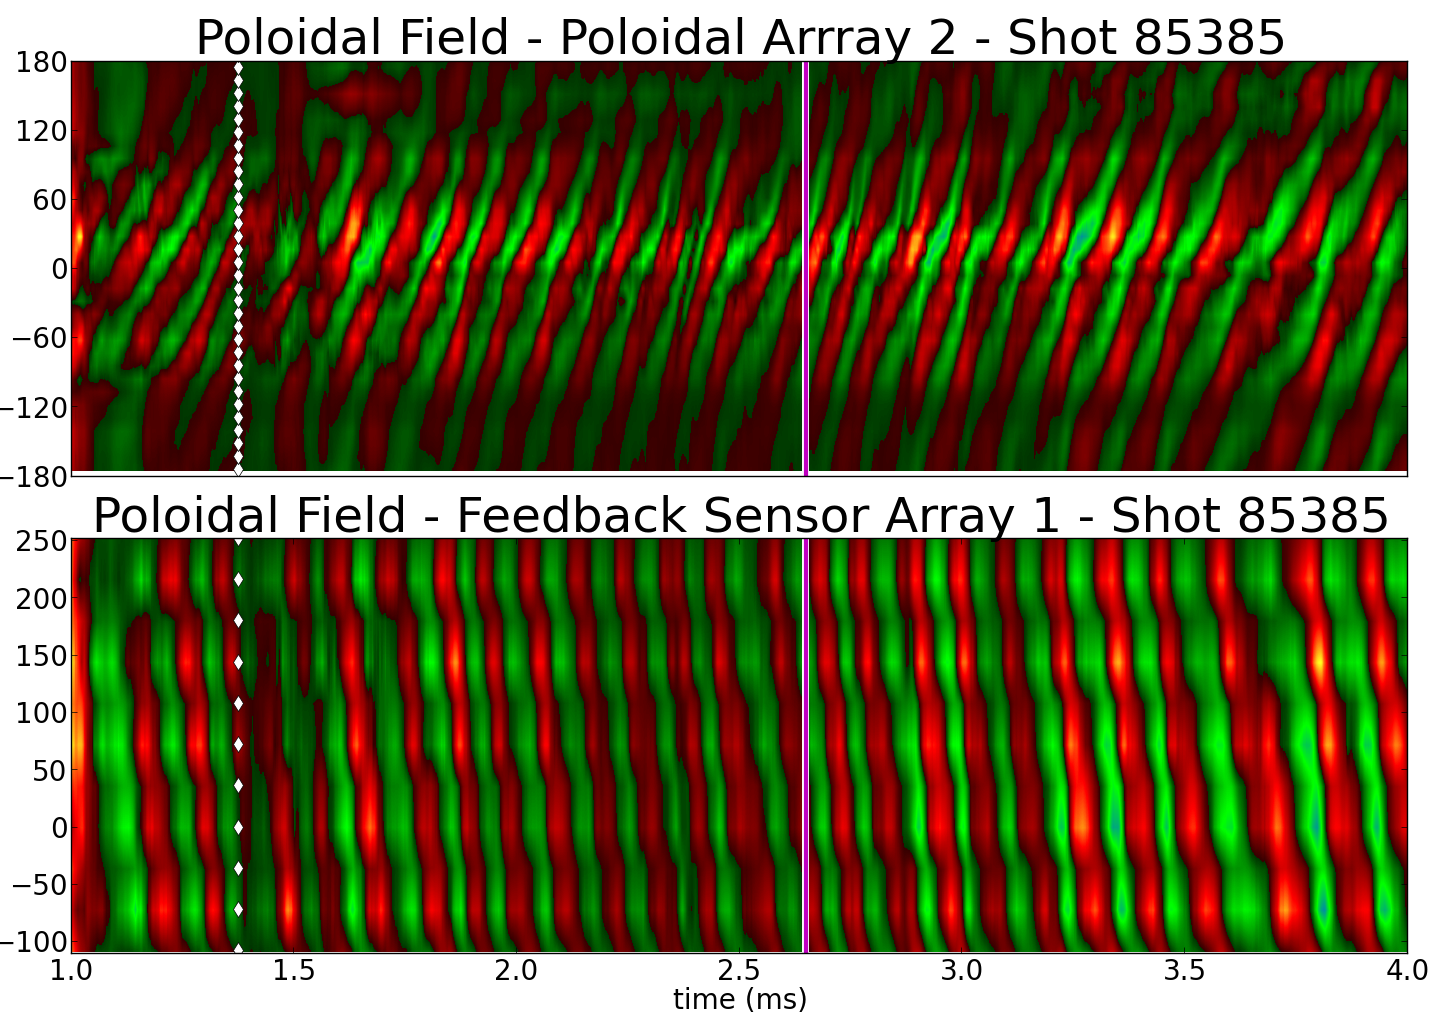
\includegraphics[scale=.25]{../Plots/stripey_plot_85385_new.png}\caption{Poloidal and Toroidal contours of perturbed poloidal field $B_\theta$ in shot 85385.  Sensors located at white circles.\\m=3, n=1 structure is visible at the time of equilibrium reconstruction (magenta line)}
\label{Stripey_85385}
\end{figure}
	We are concurrently performing studies of the effects of ferritic material on the plasma, and so those shells will be retracted and signal from sensors mounted to ferritic shells (gold panels in Fig. \ref{schematic})  will be excluded from analysis in the experiment.  This reduces to 178 the number of usable sensors, which is still a large multiple of most other experiments' resolution.
\subsection{Potential Issues}
	HBT-EP's Ohmic field has a mod-B null at the midplane with a major radius of 89cm.  Current induced by the Ohmic loop voltage will be remain in this channel, and as Ip increases, the poloidal field will be created that confines a toroidal plasma.  Initializing the shaping coils before breakdown would be inappropriate as shaping fields push the null downwards and outwards into the shells, and the effect is exacerbated by the OH field passing through zero as the current is ramped.  As such, plasma shaping cannot be imposed until after the circular plasma has formed.  Currently, the shaping field requires ~1ms to reach its peak and soak through the chamber.  This represents up to 20\% of a shaped plasma's lifetime.  By removing individual capacitors from the start bank, it will be possible to shorten this rise, if it becomes necessary.\par
	After the plasma has been formed, its vertical and radial position in the chamber is determined by the geometry of the vacuum fields.  The potential for a positional instability in which the plasma falls up, down, or out towards the walls exists if the geometry is unsuitable.  Stability is quantified in terms of a decay index of the vertical vacuum field with respect to the major radius R:$$n = -\frac{R}{B_z}\frac{\delta B_z}{\delta R}$$\par
	The criterion for vertical stability is that n be greater than zero, and for radial stability that n be less than ~1.5.  Plasmas with n outside this range will be positionally unstable, but the growth rate of the instability will be reduced in the presence of a resistive wall\cite{Fukuyama}.%  The condition for vertical stability can be expressed as:
%$$\frac{\gamma_g^2}{\Gamma_0^2} = -\left( n + n_s\frac{\gamma_g\tau_s}{1+\gamma_g\tau_s}\right)$$
%	and the condition for radial stability is:
%	$$\frac{\gamma_g^2}{\Gamma_0^2} = n - S_0 - n_s\frac{\gamma_g\tau_s}{1+\gamma_g\tau_s}$$
%	where
%	$$\tau_s = \tau_{rw}\left(1-\frac{a^2}{b^2}\right)$$
%	$$\Gamma_0^2 = \frac{\rho_0 B_p^2(a)\Lambda}{\mu_0 R^2}$$
%	$$n_s = -\frac{2 R_0^2}{\Lambda (b^2-a^2)}$$
%	$$\Lambda = ln\left(\frac{8R}{a_0}\right) + \frac{l_i -3}{2} + \bar{\beta}_{p0}$$
%	$R$ is the plasma major radius,$a$ is the minor radius, $b$ is the radius of the inner edge of the resistive shell,$\tau_{rw}$ is the skin time of the shell, $\rho_0$ is the mass density of the plasma being confined,$B_p(a)$ is the poloidal field at the plasma edge, $l_i$ is the internal inductance of the plasma, $S_0$ is ~1.5 in an air-core Tokamak, such as HBT-EP  $\bar{\beta}_{p0}$ is the volume averaged poloidal beta.\par
	%The solution of the diffusion equation leads to a resistively stabilized instability space.
	\par The growth rate in the case of instability is reduced by wall eddy currents, and while the plasma is still unstable with $n < 0$ or $n > 1.5$, the instability will not grow at speeds faster than 1kHz until $|n| > 10$.  %, as seen in Figure \ref{decay_index_stabilization}.  
	Given that shaped plasmas generally do not persist for longer than 3ms after the imposition of the full shaping field, and on disruption fall inwards, despite the instability drive pushing outwards (Figure \ref{decay_index_and growth}) it is unlikely that the positional instability is limiting the lifetime of the plasma.  If shot development leads to longer lived shaped plasmas, it may however become performance limiting.
%\begin{figure}[htb]
%\centering
%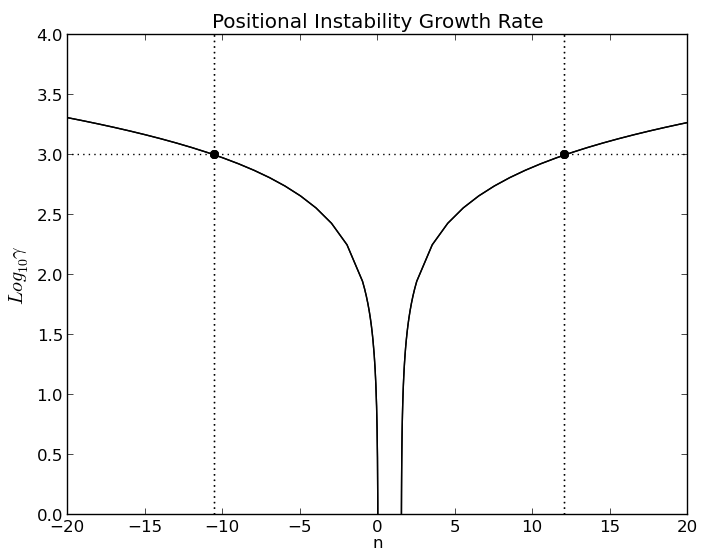
\includegraphics[scale=.45]{../Plots/Decay_growth_narrow.png}\caption{Growth rate of positional instability with decay index.  There exists a range of $-10 < n < 12$ in which the growth rate is slower than 1kHz}
%\label{decay_index_stabilization}
%\end{figure}
\begin{figure}[htb]
\centering
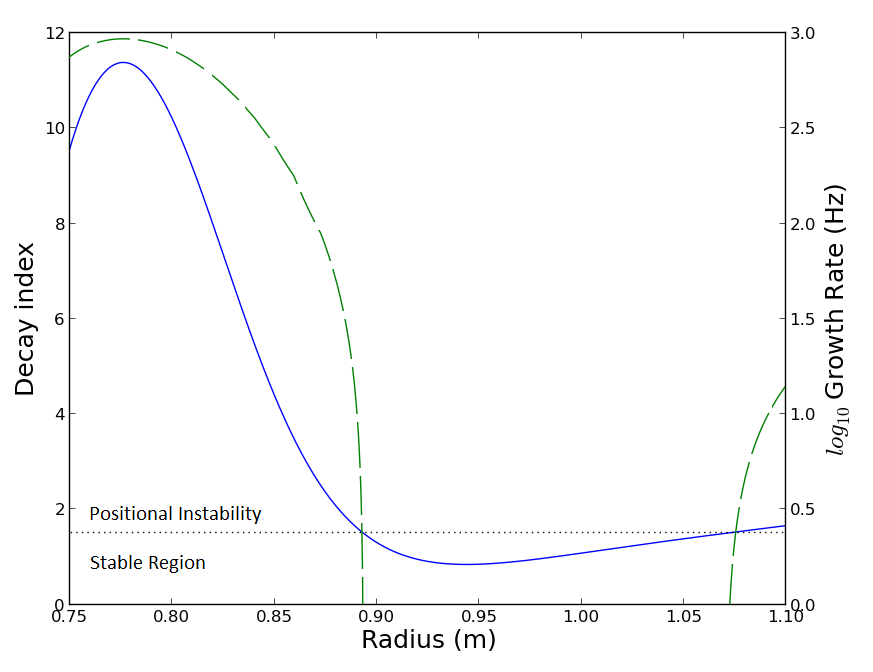
\includegraphics[scale=.375]{../Plots/Decay_stability_and_growth_on_midplane-edit.png}\caption{Areas of stability and slow growth in shot 85385 at 3.5ms. Decay index is the solid blue line, while growth rate is dashed green. Plasma is stable when n $<=$1.5.}
\label{decay_index_and growth}
\end{figure}
%	The shaping coil was installed in-situ, without disassembling the machine first.  This added to the complexity of installation and required certain compromises in the design.  The thickness of the coil's cabling, the lack of available space and high density of external ports and other obstructions on the high field side of the machine have made threading the coil in an axisymmetric manner impossible.  The field errors introduced were expected to be small, however, large differences between the measured fields on the toroidal array sensors and the two poloidal arrays, as seen in Figure \ref{fluxes and fields}, suggest that the errors were larger than anticipated.  Work is ongoing towards understanding and minimizing these errors.\par
%Fortunately, the error fields all tend to increase the coupling between the coil and plasma.  At the toroidal location where the shaping is strongest, material that lies outside the local LCFS will run to the wall and be scraped off, even if it would be within a confined plasma elsewhere, that is, assuming fast enough parallel transport, the LCFS at the location of the strongest field error will be the global LCFS.  The result is a plasma that is generally more strongly diverted than otherwise.  If the intent is to only apply a low level of shaping, the same argument applies, and it should be possible to achieve our ends by recalibrating the shaping current to account for the fact.
%	Additionally, the plasma operates in a horizontally unstable regime due to the imposition of the x-point.  We have seen the HBT-EP plasma lifetime reduced when shaping is imposed, coupled with a stronger inward major radius crash at disruption.  These effects both take place on timescales too large to be accounted for by ideal theory, though the predictions of \ref{} et. al. suggest it should be possible to extend the lifetime of the plasma further.

\section{Proposed Research}
	This document proposes to study the structure and dynamics of the shaped MHD spectrum, in the presence or absence of resistive wall  stabilization of the plasma and resonant magnetic perturbations (RMPs).  The shaping coil current will be varied to allow observation of diverted plasmas as well as shaped limited plasmas.  Detailed comparison to calculations will be made and we will determine if the shaping changes the overall behavior of a plasma discharge\par 
	\subsection{Forward Modeling of Plasma Equilibrium and MHD modes}
	Observing the MHD spectrum of a shaped HBT-EP plasma presents new challenges that must be overcome.  Many of our analysis techniques rest on an assumption of a circular plasma limited at a fixed surface.  In this case, for a given B$_T$, he only variable determining plasma shape is MR, and the only variables determining  q$^*$ are MR and Ip. Once shaping is introduced, the plasma shape, size and location of LCFS in R-Z space is a (domiantly) 3-parameter fit using Ip, Ish, and MR.  Matching a shaped equilibrium as closely as possible to an unshaped one will require forward modeling.
	Further, the sensor arrays were designed with a circular plasma in mind, and thus have a roughly constant coupling to the plasma surface.  In a shaped plasma, the sensors' coupling to the plasma will vary poloidally.  As it is primarily a modification of the spectrum in the poloidal direction, especially near the X-point, that we expect to see, we must understand and correct for how the coupling varies.\par 
	We will use HBT-EP's standard suite of simulation software, consisting of TokaMac, DCON, and VALEN for this research.  TokaMac is an equlibrium reconstruction code and will be used to determine which combination of plasma parameters will give us an equilibrium to study that is most similar to an unshaped plasma of interest.  DCON will then return the stability and shape of the plasma modes for that equilibrium, and VALEN will be used, to predict the detection of those modes as measured at our sensors.  This last method represents a novel method for HBT-EP and has already suggested ways of improving our RMP methodology.  This is discussed in a later subsection.
	\subsection{Natural Modes in Circular Limited, Shaped Limited, and Diverted Plasmas}		
	The techniques outlined above will allow us to observe the structure and evolution of natural modes in a shaped plasma, and compare them to those present in a circular one.  Mode structure, growth and saturated amplitude, as well as disruptivity will be studied and compared to standard circular plasmas. Initial shots have been taken with a constant shaping field imposed.  Assuming a stable enough plasma, a BD can be taken over a window of time in which these quantities do not vary significantly.\par
	Slightly more difficult, but still well within our capabilities, would be choosing initial conditions for the shaping power supply such that shaping current rises proportionately with the plasma current.  If the major radius remains roughly constant, the location of the last closed flux surface - and if the plasma is diverted, X-point - remain relatively fixed in space.  This would allow us to observe the modes in shaped and/or diverted plasmas with roughly constant profiles and cross-sectional shape, as we currently do with circular plasmas.  This technique would be useful as well in all following experiments\par
	%Modifications to the poloidal structure of the modes have been observed.  This is seen in Fig. \ref{Stripey_85385}, near the divertor.  The shaping coil's ramp-phase lasts from 1.5 to 2.5 ms, and residual pickup is indeed seen in the raw fluctuations at this time.  However, the boxcar smoothing rapidly improves as the shaping coil maintains its steady state value, and at 3.5 ms, there is a clear 'hitching' as a mode trough passes that area, with the peak eventually passing in a rapid, high amplitude spike.  The mode is seen to continue rotating far away, giving the appearance of the poloidal perturbation 'piling up' at the x-point as it rotates.\par
	%Not enough analysis has been done to say definitively what is occurring.  It is unlikely that the X-point is exerting a poloidally localized torque on the mode.  It is however possible that there is a second mode, highly localized at the X-point, which is interfering with the dominant mode.  Locking to error fields, which are significant (see Potential Issues below) is another factor that must be considered.  Either or both of those options could be consistent with the X-point localized kink/tearing mode\cite{Huysmans}
	\subsection{MHD Response to Driven Perturbations}
\begin{figure}[b]
	\centering
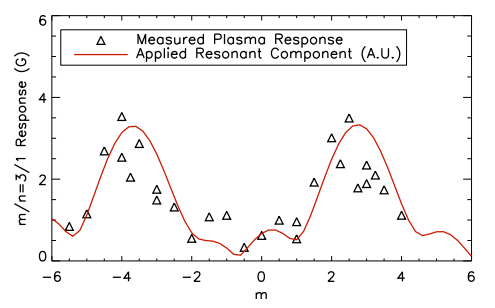
\includegraphics[scale=.525]{../Plots/Shiraki_thesis_Fig_7_1.png}\caption{Plasma response to RMPs of various helicities.  The red line represents the relative amount of +3/1 helicity in each mode.  Taken from referenece \cite{Shiraki}, Figure 7.1}
	\label{Shiraki_plot}
	\end{figure}
HBT-EP's active control saddle coils will be used to impose RMPs of varying helicities to investigate the sensitivity of a shaped or diverted plasma to resonant and non-resonant perturbations.  This has been investigated in circular plasmas previously\cite{Shiraki}.  As seen in Fig \ref{Shiraki_plot}, the 3/1 content of the imposed mode is the major factor in determining plasma response.  Whether the level of response to an RMP's 3/1 component increases or decreases, or whether the response will couple more strongly to a different helicity altogether, and how these effects vary with q* will be the main thrust of this experiment.\par
	\subsection{Effect of Resistive Wall Stabilization on natural MHD Modes}	 
HBT-EP's modular walls will be retracted or inserted to influence the amount of passive stabilization of the MHD modes.  Retracting the shells, one would expect to see the unstable MHD modes appear with faster growth rates and, possibly, larger amplitudes\cite{Shiraki}.  This should help discriminate the unstable modes from the more stable fluctuations and increase the contrast between the observed modes and background noise.  Our walls are designed to be conformal to a circular plasma, and will thus have reduced coupling to a shaped one, but assuming a shot can be developed with a constant position and shape as the shell radius is varied, we should be able to draw comparisons.  With the ferritic segments installed in the vacuum vessel, we will only be able to use 10 of the 20 shells for this experiment, but that should provide enough stabilization to discern a difference.\par
\subsection{Reversed Polarity Shaping}
The shaping coil bank was constructed in such a way that the shaping current can be reversed with ease.  Rather than creating a single-null, diverted plasma, we will create a bean-shaped, limited plasma.  We will be able to perform all the tests described for a diverted plasma on our bean-shaped plasmas.  See Figure \ref{bean_plasma_flux_and_modes} for an example equilibrium created with TokaMac.\par
By strengthening the poloidal field on the good curvature side, we will in effect reduce the average goodness of curvature for any given field line.  We should expect to see stronger, more repsonsive, and/or more disruptive modes in these plasmas.  It should in theory be possible to scan the shaping current from -7kA to +7kA, and observe the effect of shaping a plasma, from strongly bean-shaped, through circular, through the teardrop-limited shape of a weakly shaped plasma, all the way into magnetic diversion.ve 
\begin{figure}[htb]
	\centering
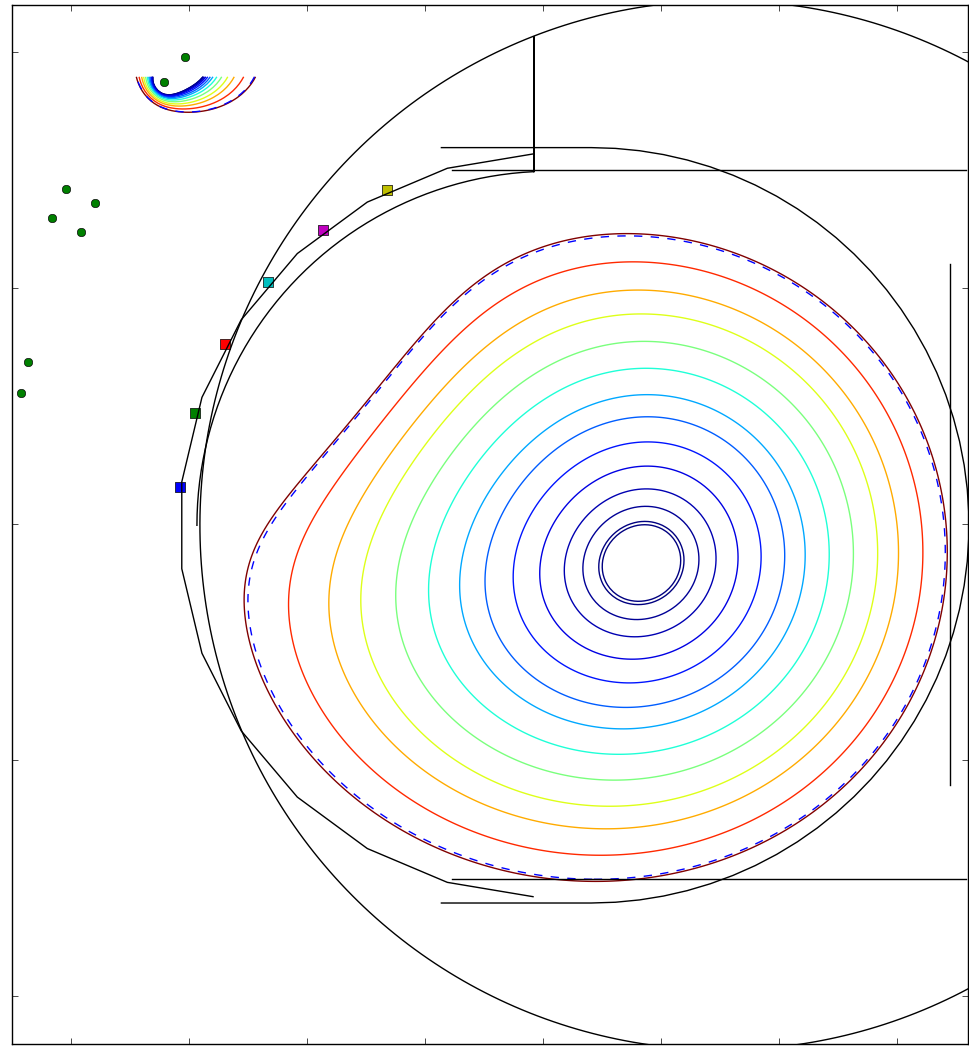
\includegraphics[scale=.22]{../Plots/bean_plasma_flux_and_currents_85385_90cm_250kPA_neg7kSH_cropped.png}\caption{Simulation of the poloidal flux surfaces of a reverse-shaped plasma}
	\label{nat_mode_sim_v_meas}
	\end{figure}
\section{Preliminary Findings}
	Several runs have been dedicated to the shaping coil since construction was finalized.  We have shaped the plasma in the presence of a variety of configurations of our passively stabilizing conducting walls, and in the presence and absence of actively driven resonant magnetic perturbations (RMPs).  We have used this work period to build a suite of analysis code, develop novel forward modeling methods, determine the safe operating parameters and determine deviations from the design. \par 
\begin{figure}[b]
	\centering
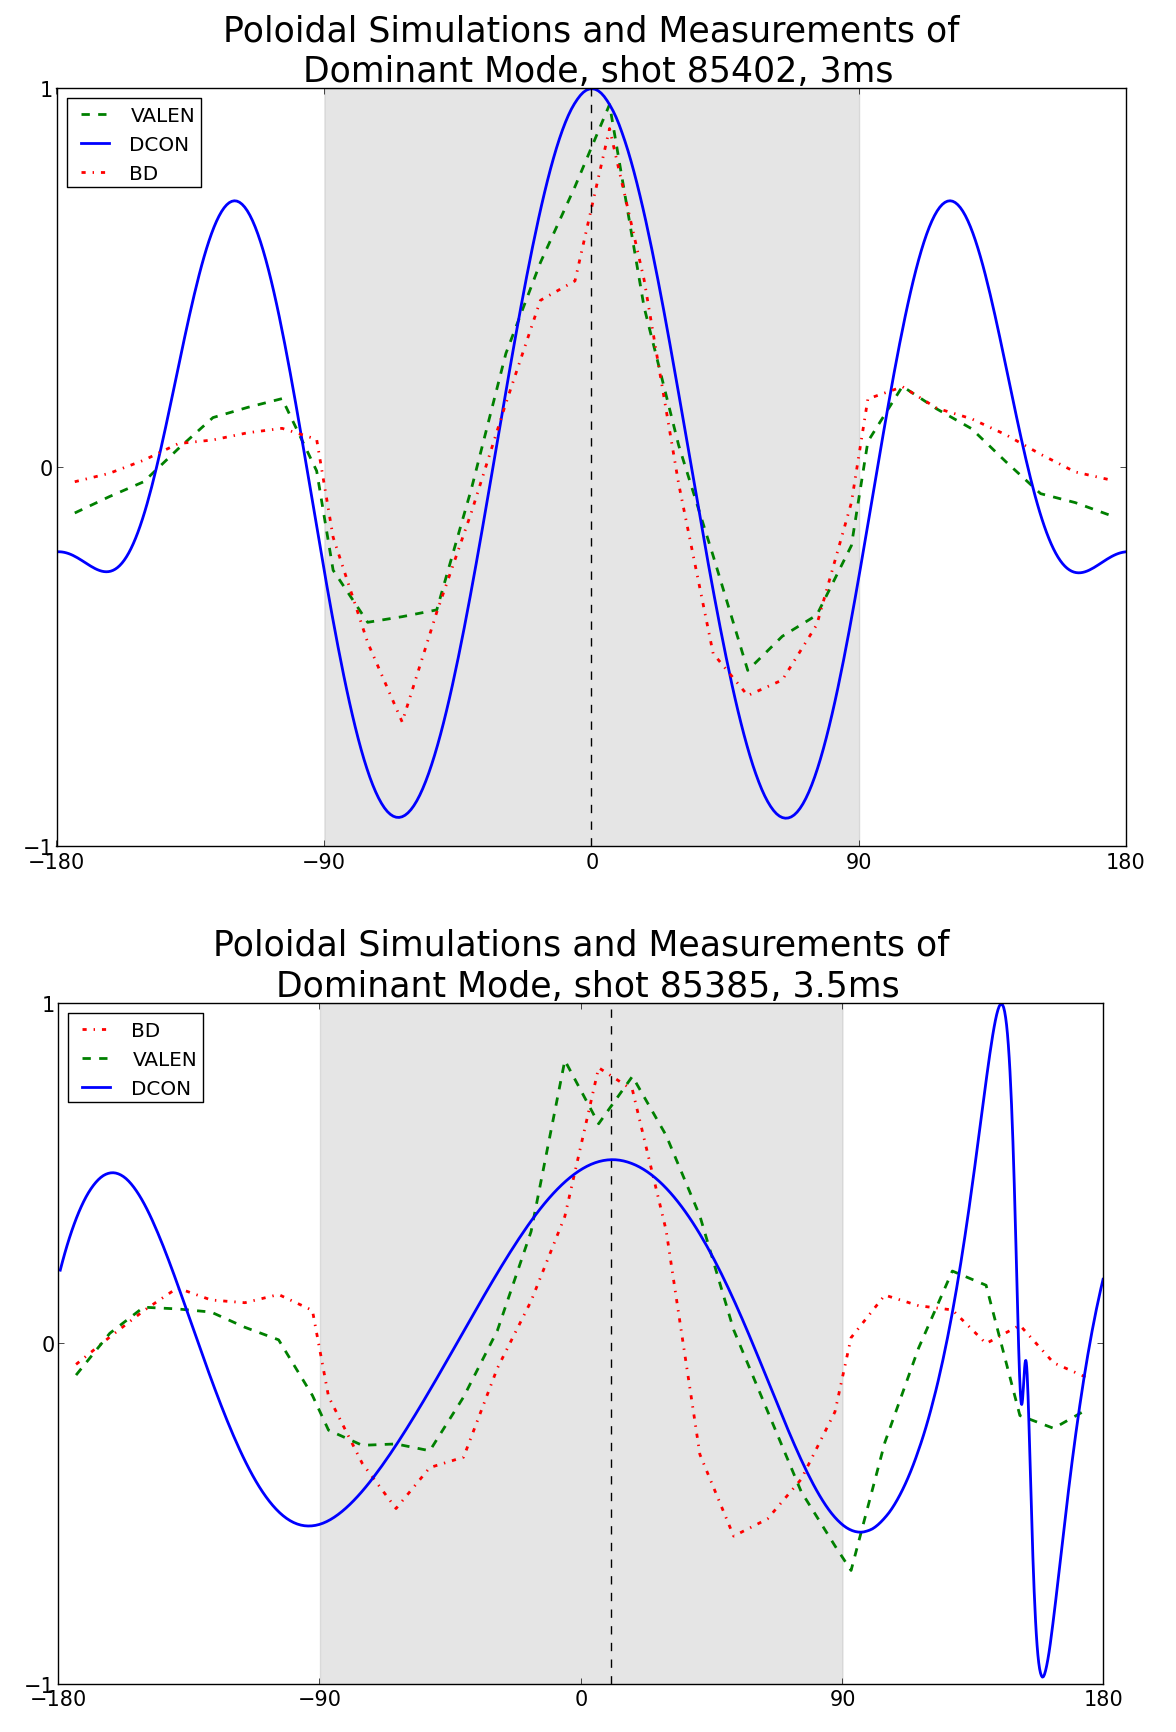
\includegraphics[scale=.22]{../Plots/DCON_VALEN_BD_comp_sh_unsh.png}\caption{Simulation of the poloidal structure of the least stable n$=$1 mode at the plasma surface by DCON, at the poloidal array sensors by VALEN, and the measured signal.\\  Poloidal angle covered by shells is shaded grey}
	\label{nat_mode_sim_v_meas}
	\end{figure}
%\begin{figure}[htb]
%	\centering
%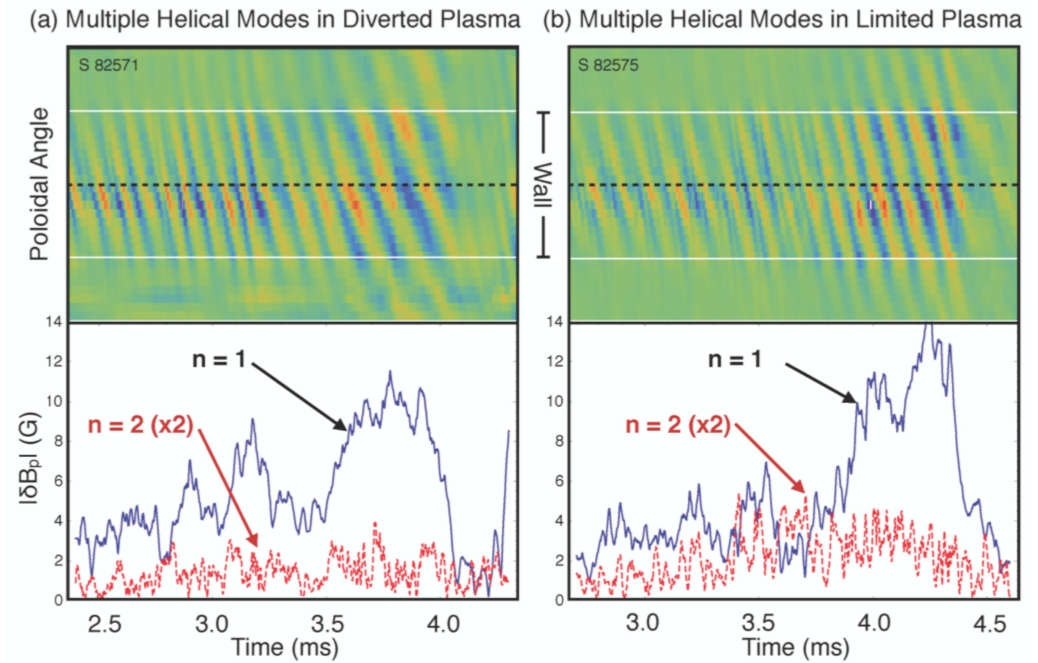
\includegraphics[scale=1]{../Plots/IAEA_plot_cropped.png}\caption{Mode content for shots 82751 (plot label is a typo) and 82575.  n=2 content is seen to be lower relative to n=1 in a shaped plasma}
%	\label{IAEA_plot}
%	\end{figure}
%\begin{figure}[htb]
%	\centering
%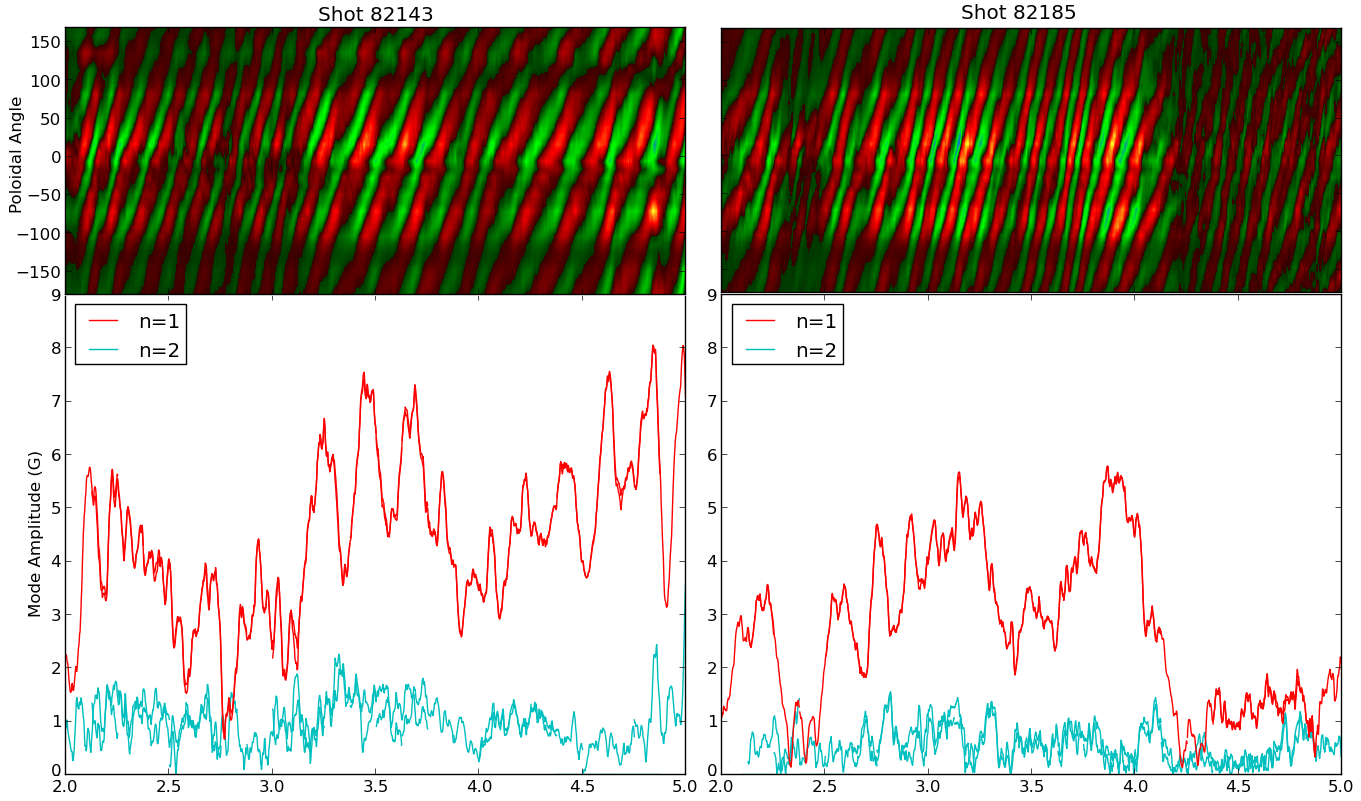
\includegraphics[scale=.25]{../Plots/82143_82185mode_amp_stripes.png}\caption{\\Mode content for shots 82143 (shaped) and 82185 (unshaped).  n=2 content is seen to be higher in a shaped discharge.}
%	\label{Modes_stripes_143_185}
%	\end{figure}

	%Thus far, the observed multi-mode behavior has followed no clear pattern.  Two pairs of shots that have been analyzed illustrate this.  Shots 82751 and 82575 are analyzed in Figure \ref{IAEA_plot}.  Contours of the plasma fluctuations in the poloidal arrays show a dominant 3-1 mode, while a (5 or 6)-2 mode can also be distinguished.  The shaped plasma seems to have the n=2 mode suppressed, while the main n=1 mode seems to rotate faster, up until the slowdown that precedes a disruption.\par
	%Shots 82143 and 82185 have different behavior, as seen in Figure \ref{Modes_stripes_143_185}.  These shots are more closely located in time, meaning chamber conditions and background pressure are likely more similar than the other pair.  MR and Ip behavior also agree more closely through the shot lifetime.  In this pair we also see the shaped plasma speed up after shaping is imposed at 2ms, slowing down again around 3ms.  However the mode in the unshaped plasma is rotating much faster than in the previous set.  We also see the n=1 mode much stronger in the shaped plasma than the unshaped, and the n=2 mode may be excited as well.  The n=1 crash in the unshaped shot correlates with edge q going above three, in agreement with theory, while the shaped plasma shows no such behavior.\par
	%The main lesson of these two shots is that HBT-EP's intrinsic shot-to-shot variability will require a large dataset, gathered in as small an interval of time as possible, to ensure that meaningful conclusions can be drawn.  During the next run campaign, replicating these shots will be a top priority.\par
	Natural modes have been detected in shaped and unshaped shots and compared to one another and simulations.  As can be seen in Figure \ref{nat_mode_sim_v_meas}, generally good agreement between prediction and measurement is found.  The poloidal signal is seen to be amplified by the shells, and there is qualitative agreement in the peak separation between the shaped case and VALEN.  % phase location of the peaks in the shaped case seems to be shifted in the direction predicted by VALEN.  
However, the differences between shaped and unshaped plasma modes as measured by our sensors are subtle, and radial signals are suppressed to a degree that a larger dataset is required to sharpen the contrast between them. , and the dataset of shaped shots to small, to make a useful comparison of those signals at present.  This has been an issue since the 2010 upgrade which replaced the shells, but may be overcome by developing shots such that the plasma edge is as close and conformal to the shells as possible.\par
	Breaking the measured signal down into its Fourier components highlights a surprising feature.  Simulations predict a broadening of the Fourier spectrum at both higher and lower m-numbers with shaping.  While the broadening is seen in experiments, it is exclusive to the higher m-numbers.  Signal attenuation with distance increases with increasing m, so low m number components should be measured with high fidelity.  This result deserves further study\par
	\begin{figure}[htb]
	\centering
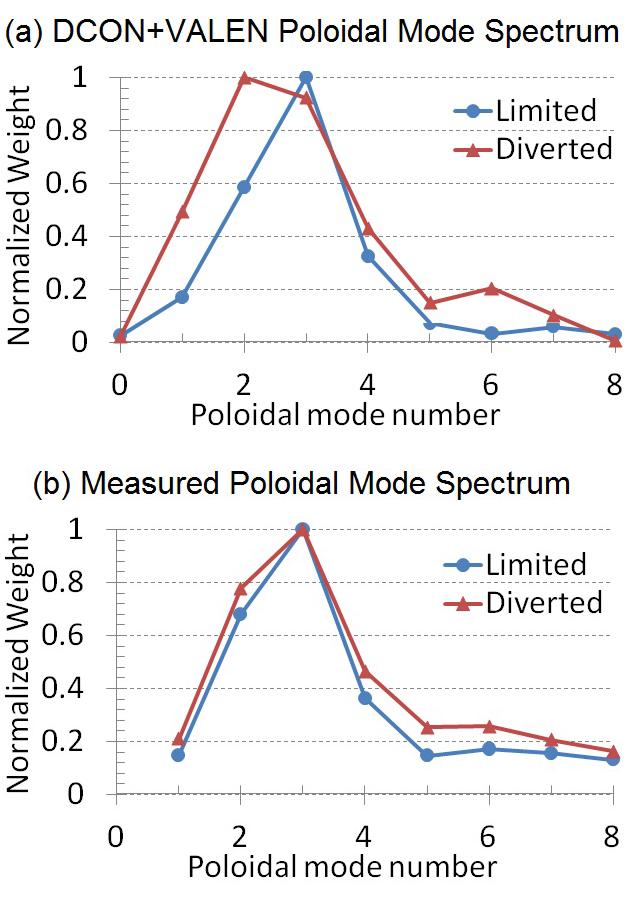
\includegraphics[scale=.5]{../Plots/fig2_mode_spectrum_REV2.png}\caption{Fourier breakdown of poloidal mode structure in shots 85402 (circular) and 85285 (shaped)}
	\label{mike_mode_structure}
	\end{figure}

3/1 RMP response has been measured using the RMP correlation method across the FBP sensors, as seen in Figure\ref{RMP_response}.  Poloidal mode structure is harder to quantify, as the largest distortion due to shaping is predicted to be located near the X-point.  The equilibrium subtraction algorithm is not yet sufficient to allow inspection of the fluctuations near the X-point due to the large equilibrum changes induced by the Shaping coil startup.  However, the poloidal structure that can be gathered from the FB signal is consistent with the mode structure predicted by the code.  Additionally, the coupling is seen to vary poloidally, which was predicted by VALEN for our non-circular, vertically offset shaped plasmas.
	
\begin{figure}[htb]
	\centering
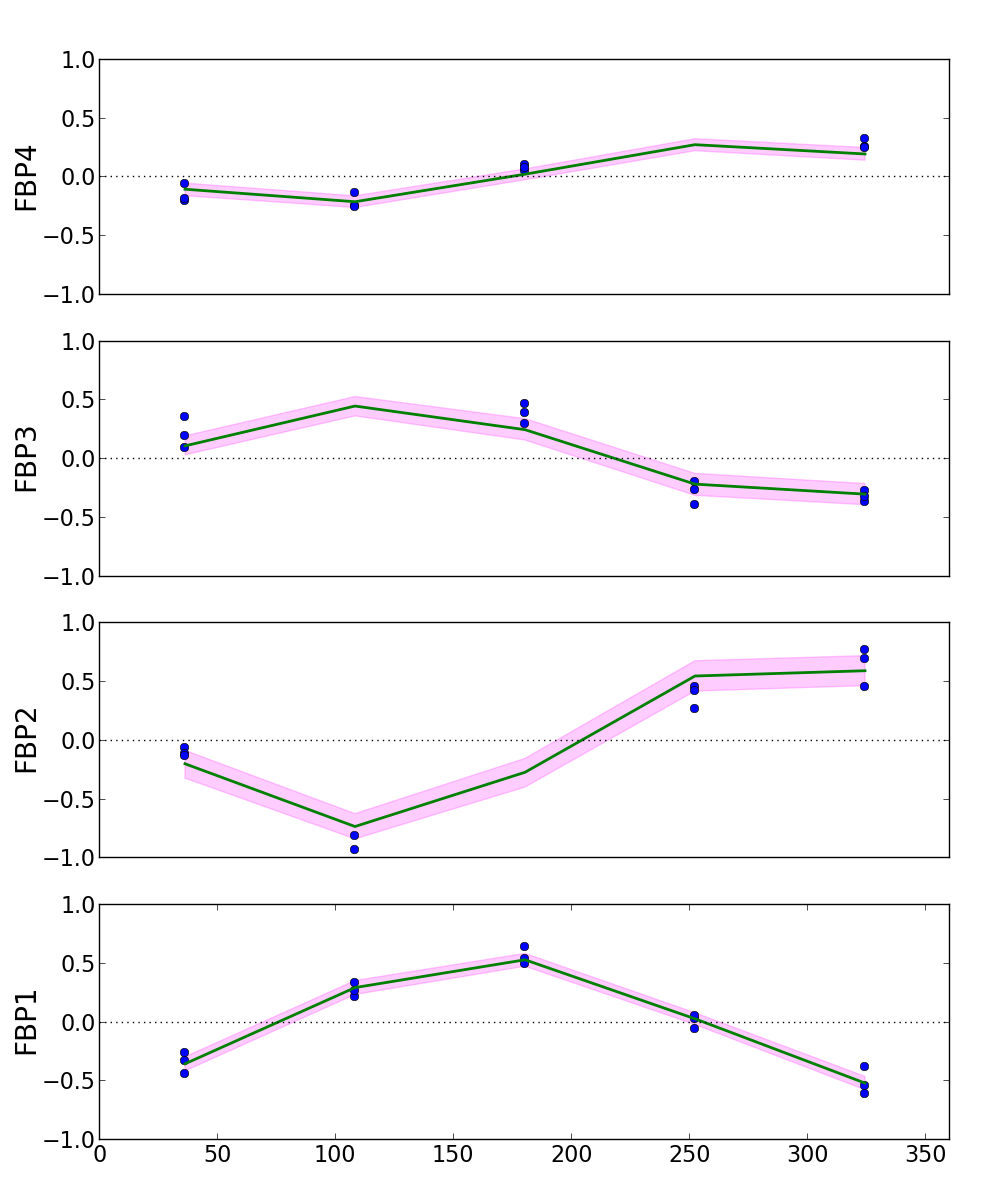
\includegraphics[scale=.35]{../Plots/response_good_plot2_84573_4_7.png}\caption{Normalized response of 3 shaped plasmas to a 3/1 RMP as measured by the 4 toroidal FB arrays.\\   ~180$^{\circ}$ of poloidal angle is covered by these arrays}
	\label{RMP_response}
	\end{figure}
	
%	DCON has also predicted changes to the natural mode structure of a shaped plasma, as seen in Figure \ref{DCON_mode_structure}.  Over and above the deformation caused by overlaying the mode on a shaped equilibrium surface, we can see that an extra zero-crossing is introduced near the x-point, and that the poloidal mode spectrum is broadened.\par
%	Direct measurements of this mode will not resemble the DCON output however.  Higher m-number modes will decay more rapidly with radial distance from the plasma surface, causing the pickup of our sensors to differ from the mode predicted by DCON.  Also, our poloidal sensors are arrayed to be conformal to a circular plasma, meaning plasma-sensor coupling will vary toroidally.  Furthermore, DCON is a purely ideal code, and does not include the effects of eddy currents in the wall and other conducting structures.  Running an analysis using VALEN to determine what signal to expect gives good agreement with the detected modes (Figure ).
\newpage
\section{Summary}
This document has proposed research into the structure and spectrum of the external kink mode in a shaped plasma utilizing HBT-EP's extensive suite of magnetic diagnostics.  To that end, a shaping coil has been built and installed on HBT-EP.  It's effect on plasma shape is localized near the coil, and gives an up-down asymmetric, diverted plasma.  The work that is to be done on this plasma is as follows:
\begin{itemize}
\item Develop a method of forward modeling the plasma equilibrium and kink mode spectrum using the three codes TokaMac, DCON and VALEN.
\item Investigate the structure and evolution of the natural modes of the diverted plasma, and compare these properties to that of a circular plasma.
\item Vary the amount of wall stabilization using HBT-EP's modular shells.  Observe the effect on both shaped and circular plasmas
\item Perturb the plasma using HBT-EP's control coil set.  Compare the response of a diverted plasma to that of a circular plasma, looking in particular at the magnitude of the response, and the location and broadness of resonant peaks.
\item In addition, these experiments will be performed at various points along the shaping parameter space, from negative-polarity shaped limited plasmas, positive polarity shaped  limited plasmas, and the aforementioned positive-polarity diverted plasmas.
\end{itemize}
\section{Acknowledgements}
Design, fabrication and installation were all aided greatly by the contributions of Nick Rivera and James Andrello.

\begin{thebibliography}{99}
%Effects on MHD due to shaping (simulations)
\bibitem{Maurer} D. A. Maurer et al., Plasma Phys. Control. Fusion, 53 (2011) 074016

%Effects on MHD due to shaping (experiment)
\bibitem{Strait} E. J. Strait, Phys. Plasmas, 1 (5) May 1994
\bibitem{Lazarus} E. A. Lazarus et al., Phys. Fluids B 3, 2220 (1991)
\bibitem{Keilhacker_HMode} M Keilhacker Plasma Phys. Control. Fusion, 29 (1987) 1401-1413

%Effects on MHD due to shaping (simulations)
\bibitem{Huysmans} G. T. A. Huysmans, Plasma Phys. Control. Fusion, 47 (2005) 2107-2121 

%Shaping coils
\bibitem{Keilhacker} M. Keilhacker et al., Nuclear Fusion Vol. 25, No. 9 (1985) 1045;

%Hardware
\bibitem{Gates} D. A. Gates, \emph{Passive Stabilization of MHD Instabilities at High ${\beta_p}$ in the HBT-EP Tokamak}, Ph.D. Thesis, Columbia University (1993).

%Decay Index
\bibitem{Fukuyama} A. Fukuyama, Japanese Journal of App. Phys., Vol. 14, No. 6 (1975) 871-77 

%MHD Theory
\bibitem{Boozer} A.H. Boozer, Phys. Plasmas (10) October 2003


%Math,Theory
\bibitem{de Wit} T. Dudok de Wit et al., Phys. Plasmas, 1 (10) October 1994
\bibitem{Levesque} J. P. Levesque, \emph{Multimode Structure of Resistive Wall Modes Near the Ideal Wall Stability Limit}, Ph.D. Thesis, Columbia University (2012).

%Mode Scraping
\bibitem{Shiraki} D. Shiraki \emph{High Resolution MHD Spectroscopy of External Kinks in a Tokamak Plasma}, Ph.D. Thesis, Columbia University (2012)

\end{thebibliography}

\end{document}
%
% ****** End of file template.aps ******
